%%%%%%%%%%%%%%%%%%%%%%%%%%%%%%%%%%%%%%%%%%%%%%%%%%%%%%%%%%%%%%%%%%%%%%%%%%%%%%%%
%2345678901234567890123456789012345678901234567890123456789012345678901234567890
%        1         2         3         4         5         6         7         8

\documentclass[letterpaper, 10 pt, conference]{ieeeconf}  % Comment this line out
                                                          % if you need a4paper
%\documentclass[a4paper, 10pt, conference]{ieeeconf}      % Use this line for a4
                                                          % paper

\IEEEoverridecommandlockouts                              % This command is only
                                                          % needed if you want to
                                                          % use the \thanks command
\overrideIEEEmargins
% See the \addtolength command later in the file to balance the column lengths
% on the last page of the document



% The following packages can be found on http:\\www.ctan.org
\usepackage{graphicx}
\usepackage{verbatim}
\usepackage{multirow}
\usepackage{rotating}
\usepackage{moreverb}                    % for boxedboxedverbatim
\usepackage{array}
\usepackage{fancyvrb}
\usepackage{multicol}
\usepackage{mdwlist}
\usepackage{enumerate}
\usepackage{fancyvrb}
\usepackage{verbatim}
\usepackage{listings}
\usepackage[usenames,dvipsnames,svgnames,table]{xcolor}

\title{\LARGE \bf
Performance Evaluation of Knowledge-based Kitting via Simulation
}
\author{Thomas Kramer$^{1}$, Zeid Kootbally$^{2}$, Stephen Balakirsky$^{3}$, Craig Schlenoff$^{4}$, Anthony Pietromartire$^{4}$, \\ and Satyandra Gupta$^{5}$% <-this % stops a space
%\thanks{*This work was not supported by any organization}% <-this % stops a space
\thanks{$^{1}$T. Kramer is with the Department of Mechanical Engineering, Catholic University of America, Washington, DC, USA
        {\tt\small thomas.kramer@nist.gov}}%
\thanks{$^{2}$Z. Kootbally is with the Department of Mechanical Engineering, University of Maryland, College Park, MD, USA
        {\tt\small zeid.kootbally@nist.gov}}
\thanks{$^{3}$S. Balakirsky is with the Georgia Tech Research Institute, Atlanta, GA
{\tt\small stephen.balakirsky@gtri.gatech.edu}}%}
\thanks{$^{4}$C. Schlenoff and A. Pietromartire are with the Intelligent Systems Division,
National Institute of Standards and Technology, Gaithersburg, MD, USA
{\tt\small craig.schlenoff@nist.gov \& pietromartire.anthony@nist.gov}}%}
\thanks{$^{5}$S. Gupta is with the Maryland Robotics Center, University of Maryland,
College Park, MD, USA
        {\tt\small skgupta@umd.edu}}%
}


\begin{document}



\maketitle
\thispagestyle{empty}
\pagestyle{empty}


%%%%%%%%%%%%%%%%%%%%%%%%%%%%%%%%%%%%%%%%%%%%%%%%%%%%%%%%%%%%%%%%%%%%%%%%%%%%%%%%
\begin{abstract}

The IEEE Robotics and Automation Society's (RAS) Ontologies for Robotics
and Automation Working Group is dedicated to developing a knowledge representation for robotics and automation. As part
of this working group, the Industrial Robots sub-group is tasked with
studying industrial applications of the knowledge representation. One of
the first areas of interest for this subgroup is the area of kit building
or kitting. This is a process that brings parts that will be used in
assembly operations together in a kit and then moves the kit to the area where the parts are used in the final assembly. It is
anticipated that utilization of the knowledge representation will allow for
the development of higher performing kitting systems. While our previous
efforts were aimed at designing the basis for performance methods and metrics that may be utilized to
determine the performance of kitting systems, this paper presents a system
that evaluates the performance of kitting systems through simulation using
specific metrics.

\end{abstract}



%%%%%%%%%%%%%%%%%%%%%%%%%%%%%%%%%%%%%%%%%%%%%%%%%%%%%%%%%%%%
\section{INTRODUCTION}
%zeid: 0.5-1 page: Industrial kitting, test methods and metrics for
% assembly from the literature review.
%Suggestion to Zeid - reference the NISTIR as a place to see the canonical
%robot commands and as a place to see a broader discussion of test methods
%for evaluating plans and plan execution.
\label{sect:Introduction}
Applications for assembly robots have been primarily implemented in fixed and programmable automation. Fixed automation is a process using mechanized machinery to perform fixed and repetitive operations in order to produce a high volume of similar parts. In programmable automation, products are made in batch quantities ranging from several dozen to several thousand units at a time. 
Although today's state-of-the-art industrial robots are capable of sub-millimeter accuracy~\cite{RobotAccuracy}, they are often programmed by an operator using crude positional controls from a teach pendant. Moreover, drastic modifications in the design process are realized when parts need major changes or become to complicated in design, thus resulting in long set up time to accommodate the new product style.

Reprogramming these robots when the aforementioned conditions arise requires that the robot cell be taken off-line for a human-led teaching period. For small batch processors or other customers who must frequently change their line configuration, this frequent down time may be unacceptable. The robotic systems of tomorrow need to be capable, flexible, and agile. These systems need to perform their duties at least as well as human counterparts, be able to be quickly re-tasked to other operations, and be able to cope with a wide variety of unexpected environmental and operational changes. In order to be successful, these systems need to combine domain expertise, knowledge of their own skills and limitations, and both semantic and geometric environmental information. The challenge of expanding industrial use of robots is through flexible automation where minimized setup times can lead in to more output and generally better throughput. Flexible robots are required to be quickly reconfigured for design and process modifications. Furthermore, they need to be information driven so that they can reliably perform different sequences of actions on command. The cost for generating the information that drives the actions must be kept down and the information must be accurate.

This paper discusses a flexible kitting system. Kitting is the process in which several different, but related items are placed into a container and supplied together as a single unit (kit). Kitting itself may be viewed as a specialization of the general bin-picking problem. In industrial assembly of manufactured products, kitting is often performed prior to final assembly. Kitting, when applied properly, has been observed to show numerous benefits for the assembly line, such as cost savings \cite{Carlsson_2008} including saving manufacturing or assembly space \cite{Medbo2003}, reducing assembly workers walking and searching times \cite{Schwind1992}, and increasing line flexibility \cite{Bozer1992} and balance \cite{Jiao2000}. In industrial assembly of manufactured products, kitting is often performed prior to final assembly. 

The increasing global competition demands the manufacturing industry to move towards state-of-the-art flexible systems. Therefore, it is important not only to know how to measure the complexity of an assembly operations -- the tasks that consist a plan -- but also to evaluate how well these operations are carried out by a manufacturing process. Recently, some theoretical measures have been explored to evaluate an assembly sequences under different contexts. For example, Sanderson and Homem de Mello~\cite{SANDERSON.1987} used the And/Or graph approach to represent feasible assembly/disassembly sequences and a function based on parts entropy measures as evaluation criteria for search in the And/Or graph space. Park \textit{et al.}~\cite{PARK.1991} described the evaluation criteria based on four evaluation functions to minimize the chances of assembly failures caused by spatial errors of parts and assembly equipment. Bonneville \textit{et al.}~\cite{BONNEVILLE.1995} presented a genetic algorithm that uses the assembly trees as model for the plans to encode them in chromosomes. The liaisons graph and the geometric constraints of the model are then used to evaluate the assembly operations. Su\'{a}rez and Lee~\cite{SUAREZ.1997} proposed a statistical measure of an assembly cost index to evaluate the assembly sequences in order to determine the optimal one.


This paper presents a system that evaluates the performance of kitting applications through simulation using specific metrics. The authors have developed a canonical robot control language (CRCL)~\cite{NISTIR.Balakirsky} that attempts to be a lowest common denominator of robot programing languages. It is anticipated that kitting plans can be translated into CRCL command sets which may then be evaluated by standardized metric software. The CRCL command sets may then be translated into a specific robot platform's language.

The organization of the remainder of this paper is as follows: Section~\ref{sect:knowledge_driven_methodology} presents an overview of the knowledge driven methodology that has been developed for this effort. Section~\ref{sect:KittingViewer} describes the Kitting Viewer tool that
simulates the execution of a plan (CRCL command file) for changing a kitting workstation from an initial state to a goal state. Section~\ref{sect:Metrics} reviews the test method and metrics that are used to compare the performance of different kitting planning systems. Section~\ref{sect:Scoring} describes a configurable scoring system that uses the five factors combined as specified by a scoring file to compute
the score of the plan and Section~\ref{sect:Conclusions} concludes this paper and discusses future work.




%%%%%%%%%%%%%%%%%%%%%%%%%%%%%%%%%%%%%%%%%%%%%%%%%%%%%%%%%%%%
%\section{DESIGN METHODOLOGY}
%zeid: 0.5-1 page

%%%%%%%%%%%%%%%%%%%%%%%%%%%%%%%%%%%%%%%%%%%%%%%%%%%%%%%%%%%%
\section{KNOWLEDGE DRIVEN METHODOLOGY}
\label{sect:knowledge_driven_methodology}
\begin{figure}[ht!]
\centering
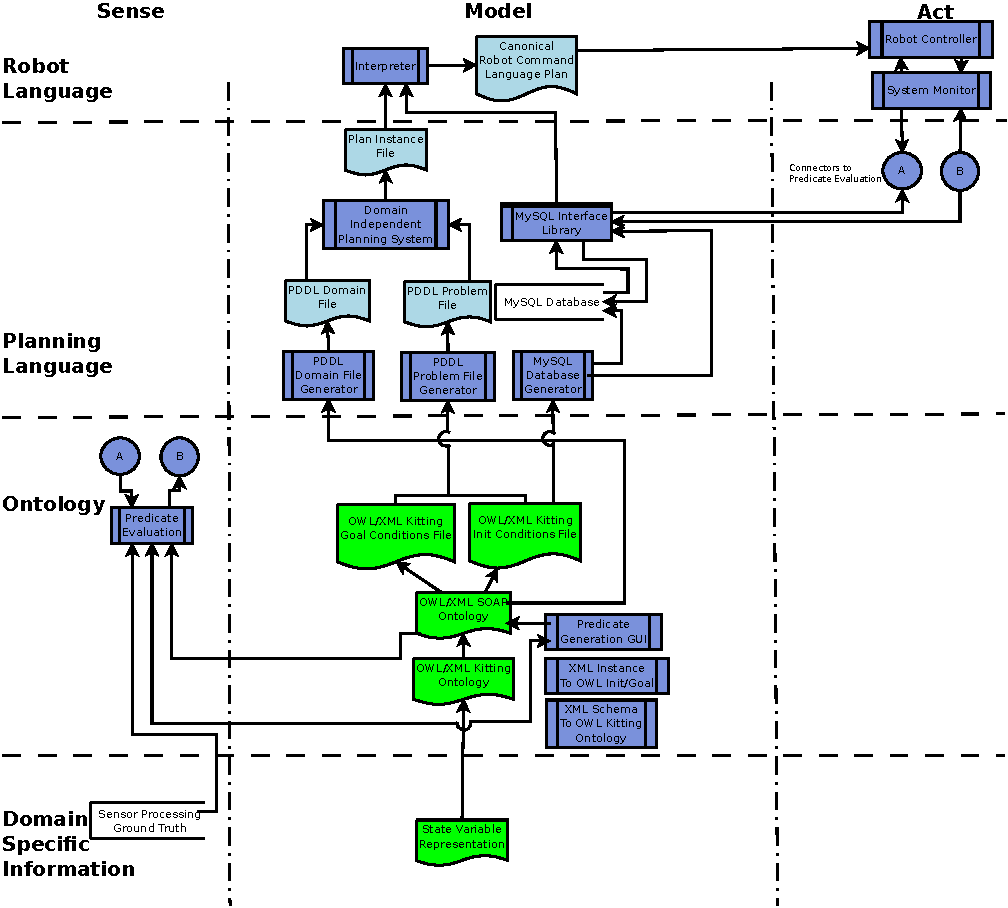
\includegraphics[width=8cm]{images/KnowledgeDrivenRobotics.pdf}
\caption{Knowledge Driven Design extensions – In this figure, green shaded boxes with
curved bottoms represent hand generated files while light blue shaded boxes with curved
bottoms represent automatically created boxes. Rectangular boxes represent processes
and libraries.
}
\label{fig:methodology}
\end{figure}
The knowledge driven methodology presented in this section is not purposed to act as a stand-alone system architecture. Rather it is intended to be an extension to well developed hierarchical, deliberative architectures such as 4D/RCS~\cite{Albus2000}. The overall knowledge driven methodology of the system is depicted in Figure~\ref{fig:methodology}. The figure is organized vertically by the representation that is used for the knowledge and horizontally by the classical sense-model-act paradigm of intelligent systems. The remainder of this section gives a brief description of each level of the hierarchy to help the reader understand the basic concepts implemented within the system architecture. The reader may find a more detailed description of each component and each level of the architecture in other documented publications~\cite{BALAKIRSKY.IROS.2012,NISTIR.Balakirsky}.

On the vertical axis, knowledge begins with Domain Specific Information (DSI) that captures operational knowledge that is necessary to be successful in the particular domain in which the system is designed to operate. This includes information on items ranging from what actions and attributes are relevant, to what the necessary conditions are for an action to occur and what the likely results of the action are. The authors have chosen to encode this basic information in a formalism know as a state variable representation~\cite{NAU.2004}.

The information encoded in the DSI is then organized into a domain independent representation. A base ontology (\textit{OWL/XML Kitting}) contains all of the basic information that was determined to be needed during the evaluation of the use cases and scenarios. The knowledge is represented in as compact of a form as possible with knowledge classes inheriting common attributes from parent classes. The \textit{OWL/XML SOAP} ontology describes not only aspects of actions and predicates but also the individual actions and predicates that are necessary for the domain under study. The instance files describe the initial and goal states for the system through the \textit{Kitting Init Conditions File} and the \textit{Kitting Goal Conditions File}, respectively. The initial state file must contain a description of the environment that is complete enough for a planning system to be able to create a valid sequence of actions that will achieve the given goal state. The goal state file only needs to contain information that is relevant to the end goal of the system. For the case of building a kit, this may simply be that a complete kit is located in a bin designed to hold completed kits.


Aspects of this knowledge are automatically extracted and encoded in a form that is optimized for a planning system to utilize (the Planning Language). The planning language used in the knowledge driven system is expressed with the Planning Domain Definition Language (PDDL)~\cite{PDDL} (version 3.0). The PDDL input format consists of two files that specify the domain and the problem. As shown in Figure~\ref{fig:methodology}, these files are automatically generated from the ontology. The domain file represents actions along with required preconditions and expected results. The problem file represents the initial state of the system and the desired goal. From these two files, a domain independent planning system~\cite{Coles.ICAPS.2010} was used to produce a static \textit{Plan Instance File}. 

Once a plan has been formulated, the knowledge is transformed into a representation that is optimized for use by a robotic system (the Robot Language). The interpreter combines knowledge from the plan with knowledge from the MySQL database to form a sequence of sequential actions that the robot controller is able to execute. The authors devised a canonical robot command language (CRCL) in which such lists can be written. The purpose of the CRCL is to provide generic commands that implement the functionality of typical industrial robots without being specific either to the language of the planning system that makes a plan or to the language used by a robot controller that executes a plan.

%written. The purpose of the CRCL is to provide generic commands that implement the functionality of typical industrial robots without being 

%specific either to the language of the planning system that makes a plan or to the language used by a robot controller that executes a plan.
%zeid: 0.5-1 page

%%%%%%%%%%%%%%%%%%%%%%%%%%%%%%%%%%%%%%%%%%%%%%%%%%%%%%%%%%%%
\section{KITTING VIEWER}
%Tom - 1 page
%currently about 2.2 pages
\label{sect:KittingViewer}
A software tool named the ``Kitting Viewer'' has been developed that
simulates the execution of a plan (CRCL command file) for changing a
kitting workstation from an initial state to a goal state. Usually, that is
a plan for making one or more kits. The Kitting Viewer evaluates the plan
as it runs. The Kitting Viewer source code is in C++ with OpenGL\footnote{Certain commercial/open source software and tools are identified in this paper in order to explain our research. Such identification does not imply
recommendation or endorsement by the authors or NIST, nor does it imply that the software tools identified are necessarily the best available for the purpose.} graphics.

\begin{figure}[ht!]
\centering
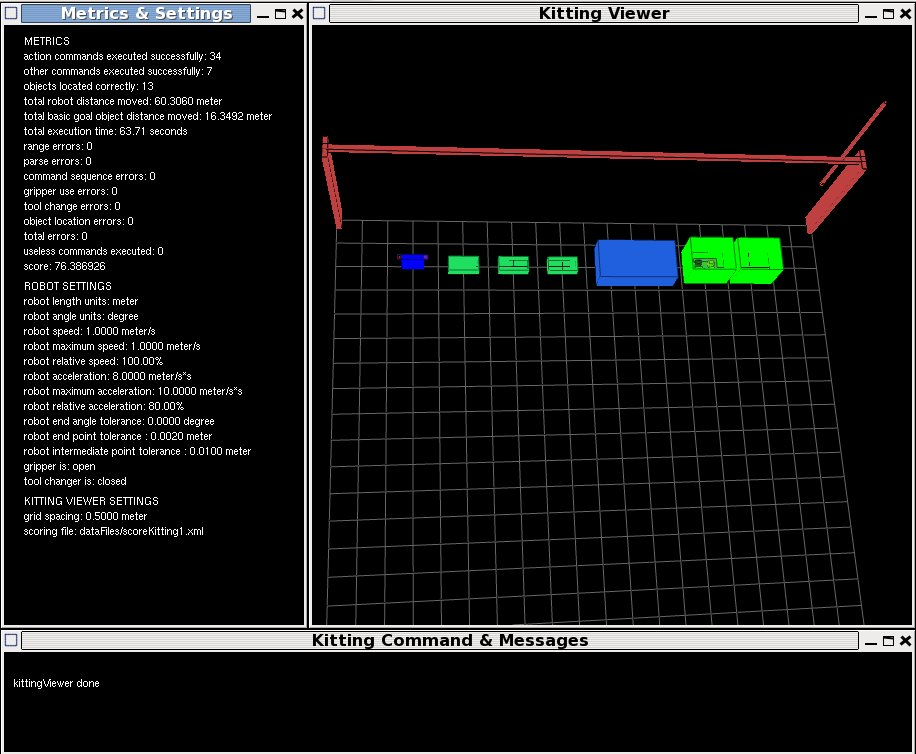
\includegraphics[width=8.5cm]{images/kittingViewer2013Feb23.jpg}
\caption{Kitting Viewer Display}
\label{fig:KittingViewer}
\end{figure}

\subsection{Overview}

The Kitting Viewer reads files describing the initial state, the goal
state, and the plan for getting from the initial state to the goal state.
Optionally, it also reads a scoring file. If no scoring file is specified
by the user, a hard-coded default scoring file structure is used. The
Kitting Viewer simulates execution of the plan, displays a view of the plan
being executed, and produces and displays metrics about the plan. All of
the metrics are numbers. All but one of the metrics are objective and
require no human judgement. These metrics are presented in Section
\ref{sect:Metrics}. The final metric is a subjective combination of the
other metrics in which the other metrics are weighted and combined as
specified by the scoring file. The scoring file may be edited as desired by
the user. Scoring details are given in Section \ref{sect:Scoring}.

Controlling the Kitting Viewer is accomplished by using the mouse and single
keys on the keyboard. When the Kitting Viewer starts up, a set of one-line
instructions is printed in the terminal window from which the
Kitting Viewer was started.

The Kitting Viewer runs in two phases. In the first phase, each time the
user gives a signal (presses the \tt g \rm key) the next command from the
command file is executed. The Kitting Viewer may decide that a command
cannot be executed, but if it decides a command can be executed, it assumes
the command is executed properly. In the second phase, which starts after
all commands have been executed, each time the user gives a signal the
position of the next movable object in the goal file is checked.

Figure~\ref{fig:KittingViewer} shows the Kitting Viewer windows as they
look after a test run has been completed. The display uses three windows,
labeled Metrics \& Settings, Kitting Viewer, and Kitting Command \&
Messages. The windows may be moved and re-sized independently, like other
windows in a typical windowing system. At any time, the user may save a
combined image of all three windows in a file in portable pixmap (.ppm)
format, a common graphics format that many graphics utilities can handle.

In Figure~\ref{fig:KittingViewer}, the large blue object is a work table.
The small blue object is the end effector changing station. The three empty
small green boxes are parts trays that formerly held parts. The large green
box on the left is a container for completed kits; it contains one kit. The
large empty green box on the right formerly held an empty kit tray.

The Kitting Viewer window shows a 3D animated color view of the kitting
workstation. The floor of the workstation is covered with a grid. The robot
in the workstation is represented by a gantry robot spanning the entire
width of the workstation. The gantry robot moves when any CRCL motion
command is executed. The speed at which the picture of the robot is
animated matches the actual commanded speed of the robot. Objects in the
workstation move if the robot moves them. The view in the window may be
translated, rotated, or zoomed at any time.

In the first phase of running the Kitting Viewer, the Kitting Command \&
Messages window shows the currently executing command or the most recently
executed command, if no command is currently executing. In the second
phase, the window shows messages describing success or failure in locating
goal objects.

The Metrics \& Settings window shows 12 (first phase) or 15 (second phase)
metrics at the top. Below that it shows 13 robot settings and two
Kitting Viewer settings. All but two of the robot settings correspond to
items that may be set using CRCL commands. The extra two are the
robot\rq{}s maximum speed and maximum acceleration, which may not be
reset. As commands are executed, metrics and settings are updated in the
window.

\subsection{Errors}
In order to fully evaluate a plan file, usually, if a plan error is
detected, an error is recorded, but the Kitting Viewer continues to operate.
A few errors are fatal.
  
When the command parser encounters a line that it cannot parse, it adds
an \sf UnreadableMsg \rm to the list of commands it has parsed. The \sf
UnreadableMsg \rm includes the text of the line on which the parse error
occurred. When the \sf UnreadableMsg \rm is executed, the value of parse
errors is increased by one and the \sf UnreadableMsg \rm is displayed in
the Kitting Command \& Messages window so the user can see the line that
caused the problem.

\subsection{Modeling}
The project in which the Kitting Viewer was developed has modeled the state
of a kitting workstation in both OWL and XML schema language. The XML model
is kitting.xsd. An automatic code generator named the GenXMiller written by
the authors at NIST is being used in the project. The GenXMiller will read
an XML schema and produce C++ classes and a parser for XML data files
corresponding to the XML schema. The GenXMiller was used to produce the C++
class model of a kitting workstation and the state file parser used in the
Kitting Viewer. The initial and goal state files used by the Kitting Viewer
are XML data files corresponding to the kitting.xsd XML schema.

The Kitting Viewer does a great deal of modeling while it runs. When the
initial state file is read, a model of the initial state is built and saved
as the current state of the workstation. A model of the goal state is also
built and saved. As the Kitting Viewer runs and CRCL commands are executed,
the Kitting Viewer determines the effect of executing each command on the
current state and updates it. The second phase of Kitting Viewer operation
compares the evolved current state with the goal state.

The logic of state changes is complex in some cases. The most interesting
cases involve what to do when executing CloseGripper and OpenGripper
commands. Details for CloseGripper are given below. 

A key issue is that composite objects may go out of existence or come into
existence while kits are being built. A kitting workstation builds kits.
The kits do not exist in the initial state but they do exist in the goal
state, so it is necessary to make them start to exist at some point in the
process. The initial state includes parts trays with parts. When all the
parts are removed from a parts tray with parts, it goes out of existence.
Of course the parts tray remains, but it is no longer a component of a
parts tray with parts. In the Kitting Viewer, a kit comes into existence
when the first part is placed in a kit tray, and a parts tray with parts
goes out of existence when the last part is removed from it.

For CloseGripper, if all of the following hold:
\newcounter{ifcount}
\begin{list}{\arabic{ifcount}.}%
{\usecounter{ifcount}}

\item  The robot is holding an end effector.

\item  The end effector is a single cup vacuum gripper (that's the only
   kind of gripper the Kitting Viewer knows how to use).

\item Either:\\
3a. There is a parts tray or kit tray with a topless boxy shape
    such that the gripper cup is within 0.1 mm of the bottom of the
    tray and is within 1 mm of the XY location of the origin of the tray. OR\\
3b. There is a part with a boxy shape with top such that the gripper cup
    is within 0.1 mm of the top of the part and is within 1 mm of the XY
    location of the middle of the top of the part.

\item The gripper is able to pick up that type of part or tray.

\item The Z axis of the gripper is 0,0,-1 and the Z axis of the object is
    0,0,1.

\item The gripper is open (implying the gripper is not holding anything).

\end{list}

Then the gripper will attach to an object. Call it B.

\begin{itemize}

\item If 3b above occurred, then B is a part

\item If 3a above occurred with a parts tray in a parts tray with parts,
   then B is the parts tray with parts.

\item If 3a above occurred with a parts tray not in a parts tray with parts,
   then B is the parts tray.

\item If 3a above occurred with a kit tray in a kit, then B is the kit.

\item If 3a above occurred with a kit tray not in a kit, then B is the kit tray.

\end{itemize}

When the gripper attaches to an object, the primary state changes (i.e.
changes in states present in kitting.xsd) are that the gripper is closed,
and the pose of the object is changed so that the object is located
relative to the gripper. In addition, as described above, if the object is
the last part in a parts tray with parts, the parts tray with parts will go
out of existence. The Kitting Viewer has several other state variables for
positions to make its work more efficient, and these are also updated.



%%%%%%%%%%%%%%%%%%%%%%%%%%%%%%%%%%%%%%%%%%%%%%%%%%%%%%%%%%%%
\section{TEST METHODS AND METRICS}
%Tom - 1 page
%currently about 1.0 page
\label{sect:Metrics}
As described in the previous section, test methods are being developed that
will be suitable for comparing the performance of different kitting
planning systems. The methods look at plans that are an ordered sequence
of actions for a robot to perform. The actions are specified in terms of
the CRCL.

A sample plan file is shown in Figure~\ref{fig:KittingPlan}. The file is
designed for exercising the kittingViewer which is described in Section \ref{sect:KittingViewer}
and is not intended to make sense
as a plan. It includes a few intentional errors.

Metrics are being developed that will test both the static performance of the planning system
(i.e., end-to-end performance of a single plan without feedback or changes) as well as the
execution performance of the system (i.e., the system is allowed to replan due to changes
in the environment or action failures). The current metrics were developed with
kitting specifically in mind. However, it is envisioned that we will eventually have
a taxonomy of metrics where high-level metrics build upon lower level metrics and
branches of the taxonomy may be applicable across multiple domains. For many
applications, it will be useful to have a single numeric score that represents a system\rq{}s
performance with respect to the individual metrics. This may be accomplished by having a
user specify whether each weight is multiplicative or accumulative and specifying
weights for each of the accumulative metrics. The metric scores are then multiplied by
these weights and combined to form a single score that may be used for comparison.

\subsection{Static Kitting Viewer Metrics}
\begin{figure}[ht!]
		\begin{center}
			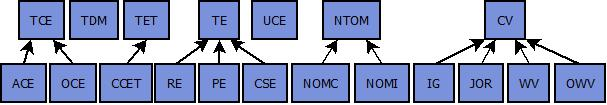
\includegraphics[width=3.1in]{images/MetricTaxonomy.jpg}
			%% Graphic for TeX using PGF
% Title: Z:\people\stephen\GlobalDocs\Projects\IPMAS\Architecture\Metric Taxonomy.dia
% Creator: Dia v0.97.2
% CreationDate: Thu Nov 01 16:39:04 2012
% For: stephen
% \usepackage{tikz}
% The following commands are not supported in PSTricks at present
% We define them conditionally, so when they are implemented,
% this pgf file will use them.
\ifx\du\undefined
  \newlength{\du}
\fi
\setlength{\du}{15\unitlength}
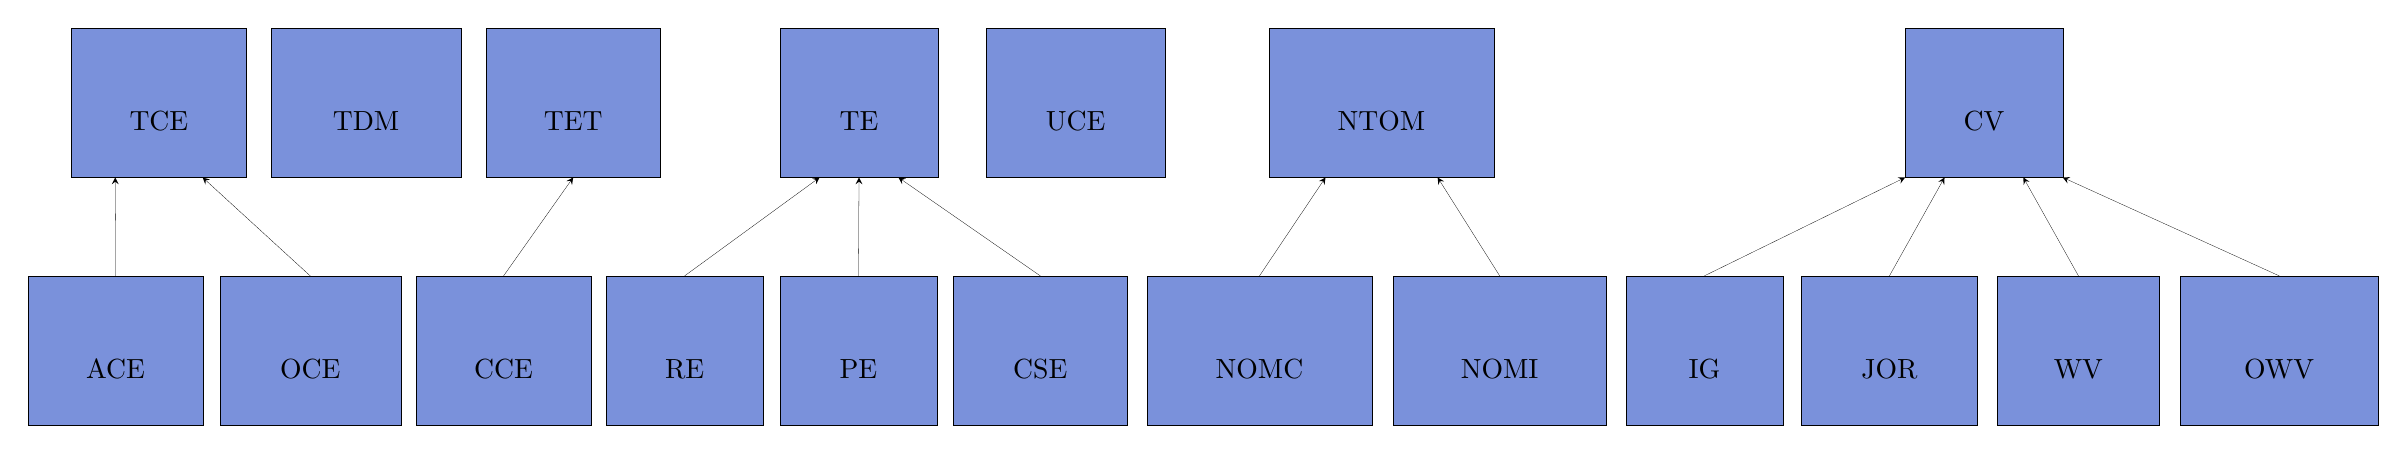
\begin{tikzpicture}
\pgftransformxscale{1.000000}
\pgftransformyscale{-1.000000}
\definecolor{dialinecolor}{rgb}{0.000000, 0.000000, 0.000000}
\pgfsetstrokecolor{dialinecolor}
\definecolor{dialinecolor}{rgb}{1.000000, 1.000000, 1.000000}
\pgfsetfillcolor{dialinecolor}
\definecolor{dialinecolor}{rgb}{0.478431, 0.568627, 0.858824}
\pgfsetfillcolor{dialinecolor}
\fill (1.257500\du,13.750000\du)--(1.257500\du,15.650000\du)--(3.487500\du,15.650000\du)--(3.487500\du,13.750000\du)--cycle;
\pgfsetlinewidth{0.100000\du}
\pgfsetdash{}{0pt}
\pgfsetdash{}{0pt}
\pgfsetmiterjoin
\definecolor{dialinecolor}{rgb}{0.000000, 0.000000, 0.000000}
\pgfsetstrokecolor{dialinecolor}
\draw (1.257500\du,13.750000\du)--(1.257500\du,15.650000\du)--(3.487500\du,15.650000\du)--(3.487500\du,13.750000\du)--cycle;
% setfont left to latex
\definecolor{dialinecolor}{rgb}{0.000000, 0.000000, 0.000000}
\pgfsetstrokecolor{dialinecolor}
\node at (2.372500\du,14.940000\du){ACE};
\definecolor{dialinecolor}{rgb}{0.478431, 0.568627, 0.858824}
\pgfsetfillcolor{dialinecolor}
\fill (3.694840\du,13.750000\du)--(3.694840\du,15.650000\du)--(5.992340\du,15.650000\du)--(5.992340\du,13.750000\du)--cycle;
\pgfsetlinewidth{0.100000\du}
\pgfsetdash{}{0pt}
\pgfsetdash{}{0pt}
\pgfsetmiterjoin
\definecolor{dialinecolor}{rgb}{0.000000, 0.000000, 0.000000}
\pgfsetstrokecolor{dialinecolor}
\draw (3.694840\du,13.750000\du)--(3.694840\du,15.650000\du)--(5.992340\du,15.650000\du)--(5.992340\du,13.750000\du)--cycle;
% setfont left to latex
\definecolor{dialinecolor}{rgb}{0.000000, 0.000000, 0.000000}
\pgfsetstrokecolor{dialinecolor}
\node at (4.843590\du,14.940000\du){OCE};
\definecolor{dialinecolor}{rgb}{0.478431, 0.568627, 0.858824}
\pgfsetfillcolor{dialinecolor}
\fill (1.812500\du,10.600000\du)--(1.812500\du,12.500000\du)--(4.032500\du,12.500000\du)--(4.032500\du,10.600000\du)--cycle;
\pgfsetlinewidth{0.100000\du}
\pgfsetdash{}{0pt}
\pgfsetdash{}{0pt}
\pgfsetmiterjoin
\definecolor{dialinecolor}{rgb}{0.000000, 0.000000, 0.000000}
\pgfsetstrokecolor{dialinecolor}
\draw (1.812500\du,10.600000\du)--(1.812500\du,12.500000\du)--(4.032500\du,12.500000\du)--(4.032500\du,10.600000\du)--cycle;
% setfont left to latex
\definecolor{dialinecolor}{rgb}{0.000000, 0.000000, 0.000000}
\pgfsetstrokecolor{dialinecolor}
\node at (2.922500\du,11.790000\du){TCE};
\definecolor{dialinecolor}{rgb}{0.478431, 0.568627, 0.858824}
\pgfsetfillcolor{dialinecolor}
\fill (4.352030\du,10.600000\du)--(4.352030\du,12.500000\du)--(6.754530\du,12.500000\du)--(6.754530\du,10.600000\du)--cycle;
\pgfsetlinewidth{0.100000\du}
\pgfsetdash{}{0pt}
\pgfsetdash{}{0pt}
\pgfsetmiterjoin
\definecolor{dialinecolor}{rgb}{0.000000, 0.000000, 0.000000}
\pgfsetstrokecolor{dialinecolor}
\draw (4.352030\du,10.600000\du)--(4.352030\du,12.500000\du)--(6.754530\du,12.500000\du)--(6.754530\du,10.600000\du)--cycle;
% setfont left to latex
\definecolor{dialinecolor}{rgb}{0.000000, 0.000000, 0.000000}
\pgfsetstrokecolor{dialinecolor}
\node at (5.553280\du,11.790000\du){TDM};
\definecolor{dialinecolor}{rgb}{0.478431, 0.568627, 0.858824}
\pgfsetfillcolor{dialinecolor}
\fill (7.074060\du,10.600000\du)--(7.074060\du,12.500000\du)--(9.294060\du,12.500000\du)--(9.294060\du,10.600000\du)--cycle;
\pgfsetlinewidth{0.100000\du}
\pgfsetdash{}{0pt}
\pgfsetdash{}{0pt}
\pgfsetmiterjoin
\definecolor{dialinecolor}{rgb}{0.000000, 0.000000, 0.000000}
\pgfsetstrokecolor{dialinecolor}
\draw (7.074060\du,10.600000\du)--(7.074060\du,12.500000\du)--(9.294060\du,12.500000\du)--(9.294060\du,10.600000\du)--cycle;
% setfont left to latex
\definecolor{dialinecolor}{rgb}{0.000000, 0.000000, 0.000000}
\pgfsetstrokecolor{dialinecolor}
\node at (8.184060\du,11.790000\du){TET};
\definecolor{dialinecolor}{rgb}{0.478431, 0.568627, 0.858824}
\pgfsetfillcolor{dialinecolor}
\fill (8.599690\du,13.750000\du)--(8.599690\du,15.650000\du)--(10.599690\du,15.650000\du)--(10.599690\du,13.750000\du)--cycle;
\pgfsetlinewidth{0.100000\du}
\pgfsetdash{}{0pt}
\pgfsetdash{}{0pt}
\pgfsetmiterjoin
\definecolor{dialinecolor}{rgb}{0.000000, 0.000000, 0.000000}
\pgfsetstrokecolor{dialinecolor}
\draw (8.599690\du,13.750000\du)--(8.599690\du,15.650000\du)--(10.599690\du,15.650000\du)--(10.599690\du,13.750000\du)--cycle;
% setfont left to latex
\definecolor{dialinecolor}{rgb}{0.000000, 0.000000, 0.000000}
\pgfsetstrokecolor{dialinecolor}
\node at (9.599690\du,14.940000\du){RE};
\definecolor{dialinecolor}{rgb}{0.478431, 0.568627, 0.858824}
\pgfsetfillcolor{dialinecolor}
\fill (10.807000\du,13.750000\du)--(10.807000\du,15.650000\du)--(12.807000\du,15.650000\du)--(12.807000\du,13.750000\du)--cycle;
\pgfsetlinewidth{0.100000\du}
\pgfsetdash{}{0pt}
\pgfsetdash{}{0pt}
\pgfsetmiterjoin
\definecolor{dialinecolor}{rgb}{0.000000, 0.000000, 0.000000}
\pgfsetstrokecolor{dialinecolor}
\draw (10.807000\du,13.750000\du)--(10.807000\du,15.650000\du)--(12.807000\du,15.650000\du)--(12.807000\du,13.750000\du)--cycle;
% setfont left to latex
\definecolor{dialinecolor}{rgb}{0.000000, 0.000000, 0.000000}
\pgfsetstrokecolor{dialinecolor}
\node at (11.807000\du,14.940000\du){PE};
\definecolor{dialinecolor}{rgb}{0.478431, 0.568627, 0.858824}
\pgfsetfillcolor{dialinecolor}
\fill (13.014400\du,13.750000\du)--(13.014400\du,15.650000\du)--(15.216900\du,15.650000\du)--(15.216900\du,13.750000\du)--cycle;
\pgfsetlinewidth{0.100000\du}
\pgfsetdash{}{0pt}
\pgfsetdash{}{0pt}
\pgfsetmiterjoin
\definecolor{dialinecolor}{rgb}{0.000000, 0.000000, 0.000000}
\pgfsetstrokecolor{dialinecolor}
\draw (13.014400\du,13.750000\du)--(13.014400\du,15.650000\du)--(15.216900\du,15.650000\du)--(15.216900\du,13.750000\du)--cycle;
% setfont left to latex
\definecolor{dialinecolor}{rgb}{0.000000, 0.000000, 0.000000}
\pgfsetstrokecolor{dialinecolor}
\node at (14.115650\du,14.940000\du){CSE};
\definecolor{dialinecolor}{rgb}{0.478431, 0.568627, 0.858824}
\pgfsetfillcolor{dialinecolor}
\fill (10.813600\du,10.600000\du)--(10.813600\du,12.500000\du)--(12.813600\du,12.500000\du)--(12.813600\du,10.600000\du)--cycle;
\pgfsetlinewidth{0.100000\du}
\pgfsetdash{}{0pt}
\pgfsetdash{}{0pt}
\pgfsetmiterjoin
\definecolor{dialinecolor}{rgb}{0.000000, 0.000000, 0.000000}
\pgfsetstrokecolor{dialinecolor}
\draw (10.813600\du,10.600000\du)--(10.813600\du,12.500000\du)--(12.813600\du,12.500000\du)--(12.813600\du,10.600000\du)--cycle;
% setfont left to latex
\definecolor{dialinecolor}{rgb}{0.000000, 0.000000, 0.000000}
\pgfsetstrokecolor{dialinecolor}
\node at (11.813600\du,11.790000\du){TE};
\definecolor{dialinecolor}{rgb}{0.478431, 0.568627, 0.858824}
\pgfsetfillcolor{dialinecolor}
\fill (13.433100\du,10.600000\du)--(13.433100\du,12.500000\du)--(15.698100\du,12.500000\du)--(15.698100\du,10.600000\du)--cycle;
\pgfsetlinewidth{0.100000\du}
\pgfsetdash{}{0pt}
\pgfsetdash{}{0pt}
\pgfsetmiterjoin
\definecolor{dialinecolor}{rgb}{0.000000, 0.000000, 0.000000}
\pgfsetstrokecolor{dialinecolor}
\draw (13.433100\du,10.600000\du)--(13.433100\du,12.500000\du)--(15.698100\du,12.500000\du)--(15.698100\du,10.600000\du)--cycle;
% setfont left to latex
\definecolor{dialinecolor}{rgb}{0.000000, 0.000000, 0.000000}
\pgfsetstrokecolor{dialinecolor}
\node at (14.565600\du,11.790000\du){UCE};
\pgfsetlinewidth{0.100000\du}
\pgfsetdash{}{0pt}
\pgfsetdash{}{0pt}
\pgfsetbuttcap
{
\definecolor{dialinecolor}{rgb}{0.000000, 0.000000, 0.000000}
\pgfsetfillcolor{dialinecolor}
% was here!!!
\pgfsetarrowsend{stealth}
\definecolor{dialinecolor}{rgb}{0.000000, 0.000000, 0.000000}
\pgfsetstrokecolor{dialinecolor}
\draw (2.372500\du,13.750000\du)--(2.367500\du,12.500000\du);
}
\pgfsetlinewidth{0.100000\du}
\pgfsetdash{}{0pt}
\pgfsetdash{}{0pt}
\pgfsetbuttcap
{
\definecolor{dialinecolor}{rgb}{0.000000, 0.000000, 0.000000}
\pgfsetfillcolor{dialinecolor}
% was here!!!
\pgfsetarrowsend{stealth}
\definecolor{dialinecolor}{rgb}{0.000000, 0.000000, 0.000000}
\pgfsetstrokecolor{dialinecolor}
\draw (4.843590\du,13.750000\du)--(3.477500\du,12.500000\du);
}
\pgfsetlinewidth{0.100000\du}
\pgfsetdash{}{0pt}
\pgfsetdash{}{0pt}
\pgfsetbuttcap
{
\definecolor{dialinecolor}{rgb}{0.000000, 0.000000, 0.000000}
\pgfsetfillcolor{dialinecolor}
% was here!!!
\pgfsetarrowsend{stealth}
\definecolor{dialinecolor}{rgb}{0.000000, 0.000000, 0.000000}
\pgfsetstrokecolor{dialinecolor}
\draw (9.599690\du,13.750000\du)--(11.313600\du,12.500000\du);
}
\pgfsetlinewidth{0.100000\du}
\pgfsetdash{}{0pt}
\pgfsetdash{}{0pt}
\pgfsetbuttcap
{
\definecolor{dialinecolor}{rgb}{0.000000, 0.000000, 0.000000}
\pgfsetfillcolor{dialinecolor}
% was here!!!
\pgfsetarrowsend{stealth}
\definecolor{dialinecolor}{rgb}{0.000000, 0.000000, 0.000000}
\pgfsetstrokecolor{dialinecolor}
\draw (11.807000\du,13.750000\du)--(11.813600\du,12.500000\du);
}
\pgfsetlinewidth{0.100000\du}
\pgfsetdash{}{0pt}
\pgfsetdash{}{0pt}
\pgfsetbuttcap
{
\definecolor{dialinecolor}{rgb}{0.000000, 0.000000, 0.000000}
\pgfsetfillcolor{dialinecolor}
% was here!!!
\pgfsetarrowsend{stealth}
\definecolor{dialinecolor}{rgb}{0.000000, 0.000000, 0.000000}
\pgfsetstrokecolor{dialinecolor}
\draw (14.115650\du,13.750000\du)--(12.313600\du,12.500000\du);
}
\definecolor{dialinecolor}{rgb}{0.478431, 0.568627, 0.858824}
\pgfsetfillcolor{dialinecolor}
\fill (6.185000\du,13.750000\du)--(6.185000\du,15.650000\du)--(8.415000\du,15.650000\du)--(8.415000\du,13.750000\du)--cycle;
\pgfsetlinewidth{0.100000\du}
\pgfsetdash{}{0pt}
\pgfsetdash{}{0pt}
\pgfsetmiterjoin
\definecolor{dialinecolor}{rgb}{0.000000, 0.000000, 0.000000}
\pgfsetstrokecolor{dialinecolor}
\draw (6.185000\du,13.750000\du)--(6.185000\du,15.650000\du)--(8.415000\du,15.650000\du)--(8.415000\du,13.750000\du)--cycle;
% setfont left to latex
\definecolor{dialinecolor}{rgb}{0.000000, 0.000000, 0.000000}
\pgfsetstrokecolor{dialinecolor}
\node at (7.300000\du,14.940000\du){CCE};
\pgfsetlinewidth{0.100000\du}
\pgfsetdash{}{0pt}
\pgfsetdash{}{0pt}
\pgfsetbuttcap
{
\definecolor{dialinecolor}{rgb}{0.000000, 0.000000, 0.000000}
\pgfsetfillcolor{dialinecolor}
% was here!!!
\pgfsetarrowsend{stealth}
\definecolor{dialinecolor}{rgb}{0.000000, 0.000000, 0.000000}
\pgfsetstrokecolor{dialinecolor}
\draw (7.300000\du,13.750000\du)--(8.184060\du,12.500000\du);
}
\definecolor{dialinecolor}{rgb}{0.478431, 0.568627, 0.858824}
\pgfsetfillcolor{dialinecolor}
\fill (15.471250\du,13.750000\du)--(15.471250\du,15.650000\du)--(18.328750\du,15.650000\du)--(18.328750\du,13.750000\du)--cycle;
\pgfsetlinewidth{0.100000\du}
\pgfsetdash{}{0pt}
\pgfsetdash{}{0pt}
\pgfsetmiterjoin
\definecolor{dialinecolor}{rgb}{0.000000, 0.000000, 0.000000}
\pgfsetstrokecolor{dialinecolor}
\draw (15.471250\du,13.750000\du)--(15.471250\du,15.650000\du)--(18.328750\du,15.650000\du)--(18.328750\du,13.750000\du)--cycle;
% setfont left to latex
\definecolor{dialinecolor}{rgb}{0.000000, 0.000000, 0.000000}
\pgfsetstrokecolor{dialinecolor}
\node at (16.900000\du,14.940000\du){NOMC};
\definecolor{dialinecolor}{rgb}{0.478431, 0.568627, 0.858824}
\pgfsetfillcolor{dialinecolor}
\fill (18.593750\du,13.750000\du)--(18.593750\du,15.650000\du)--(21.306250\du,15.650000\du)--(21.306250\du,13.750000\du)--cycle;
\pgfsetlinewidth{0.100000\du}
\pgfsetdash{}{0pt}
\pgfsetdash{}{0pt}
\pgfsetmiterjoin
\definecolor{dialinecolor}{rgb}{0.000000, 0.000000, 0.000000}
\pgfsetstrokecolor{dialinecolor}
\draw (18.593750\du,13.750000\du)--(18.593750\du,15.650000\du)--(21.306250\du,15.650000\du)--(21.306250\du,13.750000\du)--cycle;
% setfont left to latex
\definecolor{dialinecolor}{rgb}{0.000000, 0.000000, 0.000000}
\pgfsetstrokecolor{dialinecolor}
\node at (19.950000\du,14.940000\du){NOMI};
\definecolor{dialinecolor}{rgb}{0.478431, 0.568627, 0.858824}
\pgfsetfillcolor{dialinecolor}
\fill (17.026250\du,10.600000\du)--(17.026250\du,12.500000\du)--(19.873750\du,12.500000\du)--(19.873750\du,10.600000\du)--cycle;
\pgfsetlinewidth{0.100000\du}
\pgfsetdash{}{0pt}
\pgfsetdash{}{0pt}
\pgfsetmiterjoin
\definecolor{dialinecolor}{rgb}{0.000000, 0.000000, 0.000000}
\pgfsetstrokecolor{dialinecolor}
\draw (17.026250\du,10.600000\du)--(17.026250\du,12.500000\du)--(19.873750\du,12.500000\du)--(19.873750\du,10.600000\du)--cycle;
% setfont left to latex
\definecolor{dialinecolor}{rgb}{0.000000, 0.000000, 0.000000}
\pgfsetstrokecolor{dialinecolor}
\node at (18.450000\du,11.790000\du){NTOM};
\definecolor{dialinecolor}{rgb}{0.478431, 0.568627, 0.858824}
\pgfsetfillcolor{dialinecolor}
\fill (21.550000\du,13.750000\du)--(21.550000\du,15.650000\du)--(23.550000\du,15.650000\du)--(23.550000\du,13.750000\du)--cycle;
\pgfsetlinewidth{0.100000\du}
\pgfsetdash{}{0pt}
\pgfsetdash{}{0pt}
\pgfsetmiterjoin
\definecolor{dialinecolor}{rgb}{0.000000, 0.000000, 0.000000}
\pgfsetstrokecolor{dialinecolor}
\draw (21.550000\du,13.750000\du)--(21.550000\du,15.650000\du)--(23.550000\du,15.650000\du)--(23.550000\du,13.750000\du)--cycle;
% setfont left to latex
\definecolor{dialinecolor}{rgb}{0.000000, 0.000000, 0.000000}
\pgfsetstrokecolor{dialinecolor}
\node at (22.550000\du,14.940000\du){IG};
\definecolor{dialinecolor}{rgb}{0.478431, 0.568627, 0.858824}
\pgfsetfillcolor{dialinecolor}
\fill (23.783750\du,13.750000\du)--(23.783750\du,15.650000\du)--(26.016250\du,15.650000\du)--(26.016250\du,13.750000\du)--cycle;
\pgfsetlinewidth{0.100000\du}
\pgfsetdash{}{0pt}
\pgfsetdash{}{0pt}
\pgfsetmiterjoin
\definecolor{dialinecolor}{rgb}{0.000000, 0.000000, 0.000000}
\pgfsetstrokecolor{dialinecolor}
\draw (23.783750\du,13.750000\du)--(23.783750\du,15.650000\du)--(26.016250\du,15.650000\du)--(26.016250\du,13.750000\du)--cycle;
% setfont left to latex
\definecolor{dialinecolor}{rgb}{0.000000, 0.000000, 0.000000}
\pgfsetstrokecolor{dialinecolor}
\node at (24.900000\du,14.940000\du){JOR};
\definecolor{dialinecolor}{rgb}{0.478431, 0.568627, 0.858824}
\pgfsetfillcolor{dialinecolor}
\fill (26.268750\du,13.750000\du)--(26.268750\du,15.650000\du)--(28.331250\du,15.650000\du)--(28.331250\du,13.750000\du)--cycle;
\pgfsetlinewidth{0.100000\du}
\pgfsetdash{}{0pt}
\pgfsetdash{}{0pt}
\pgfsetmiterjoin
\definecolor{dialinecolor}{rgb}{0.000000, 0.000000, 0.000000}
\pgfsetstrokecolor{dialinecolor}
\draw (26.268750\du,13.750000\du)--(26.268750\du,15.650000\du)--(28.331250\du,15.650000\du)--(28.331250\du,13.750000\du)--cycle;
% setfont left to latex
\definecolor{dialinecolor}{rgb}{0.000000, 0.000000, 0.000000}
\pgfsetstrokecolor{dialinecolor}
\node at (27.300000\du,14.940000\du){WV};
\definecolor{dialinecolor}{rgb}{0.478431, 0.568627, 0.858824}
\pgfsetfillcolor{dialinecolor}
\fill (28.593750\du,13.750000\du)--(28.593750\du,15.650000\du)--(31.106250\du,15.650000\du)--(31.106250\du,13.750000\du)--cycle;
\pgfsetlinewidth{0.100000\du}
\pgfsetdash{}{0pt}
\pgfsetdash{}{0pt}
\pgfsetmiterjoin
\definecolor{dialinecolor}{rgb}{0.000000, 0.000000, 0.000000}
\pgfsetstrokecolor{dialinecolor}
\draw (28.593750\du,13.750000\du)--(28.593750\du,15.650000\du)--(31.106250\du,15.650000\du)--(31.106250\du,13.750000\du)--cycle;
% setfont left to latex
\definecolor{dialinecolor}{rgb}{0.000000, 0.000000, 0.000000}
\pgfsetstrokecolor{dialinecolor}
\node at (29.850000\du,14.940000\du){OWV};
\definecolor{dialinecolor}{rgb}{0.478431, 0.568627, 0.858824}
\pgfsetfillcolor{dialinecolor}
\fill (25.100000\du,10.600000\du)--(25.100000\du,12.500000\du)--(27.100000\du,12.500000\du)--(27.100000\du,10.600000\du)--cycle;
\pgfsetlinewidth{0.100000\du}
\pgfsetdash{}{0pt}
\pgfsetdash{}{0pt}
\pgfsetmiterjoin
\definecolor{dialinecolor}{rgb}{0.000000, 0.000000, 0.000000}
\pgfsetstrokecolor{dialinecolor}
\draw (25.100000\du,10.600000\du)--(25.100000\du,12.500000\du)--(27.100000\du,12.500000\du)--(27.100000\du,10.600000\du)--cycle;
% setfont left to latex
\definecolor{dialinecolor}{rgb}{0.000000, 0.000000, 0.000000}
\pgfsetstrokecolor{dialinecolor}
\node at (26.100000\du,11.790000\du){CV};
\pgfsetlinewidth{0.100000\du}
\pgfsetdash{}{0pt}
\pgfsetdash{}{0pt}
\pgfsetbuttcap
{
\definecolor{dialinecolor}{rgb}{0.000000, 0.000000, 0.000000}
\pgfsetfillcolor{dialinecolor}
% was here!!!
\pgfsetarrowsend{stealth}
\definecolor{dialinecolor}{rgb}{0.000000, 0.000000, 0.000000}
\pgfsetstrokecolor{dialinecolor}
\draw (16.900000\du,13.750000\du)--(17.738125\du,12.500000\du);
}
\pgfsetlinewidth{0.100000\du}
\pgfsetdash{}{0pt}
\pgfsetdash{}{0pt}
\pgfsetbuttcap
{
\definecolor{dialinecolor}{rgb}{0.000000, 0.000000, 0.000000}
\pgfsetfillcolor{dialinecolor}
% was here!!!
\pgfsetarrowsend{stealth}
\definecolor{dialinecolor}{rgb}{0.000000, 0.000000, 0.000000}
\pgfsetstrokecolor{dialinecolor}
\draw (19.950000\du,13.750000\du)--(19.161875\du,12.500000\du);
}
\pgfsetlinewidth{0.100000\du}
\pgfsetdash{}{0pt}
\pgfsetdash{}{0pt}
\pgfsetbuttcap
{
\definecolor{dialinecolor}{rgb}{0.000000, 0.000000, 0.000000}
\pgfsetfillcolor{dialinecolor}
% was here!!!
\pgfsetarrowsend{stealth}
\definecolor{dialinecolor}{rgb}{0.000000, 0.000000, 0.000000}
\pgfsetstrokecolor{dialinecolor}
\draw (22.550000\du,13.750000\du)--(25.100000\du,12.500000\du);
}
\pgfsetlinewidth{0.100000\du}
\pgfsetdash{}{0pt}
\pgfsetdash{}{0pt}
\pgfsetbuttcap
{
\definecolor{dialinecolor}{rgb}{0.000000, 0.000000, 0.000000}
\pgfsetfillcolor{dialinecolor}
% was here!!!
\pgfsetarrowsend{stealth}
\definecolor{dialinecolor}{rgb}{0.000000, 0.000000, 0.000000}
\pgfsetstrokecolor{dialinecolor}
\draw (24.900000\du,13.750000\du)--(25.600000\du,12.500000\du);
}
\pgfsetlinewidth{0.100000\du}
\pgfsetdash{}{0pt}
\pgfsetdash{}{0pt}
\pgfsetbuttcap
{
\definecolor{dialinecolor}{rgb}{0.000000, 0.000000, 0.000000}
\pgfsetfillcolor{dialinecolor}
% was here!!!
\pgfsetarrowsend{stealth}
\definecolor{dialinecolor}{rgb}{0.000000, 0.000000, 0.000000}
\pgfsetstrokecolor{dialinecolor}
\draw (27.300000\du,13.750000\du)--(26.600000\du,12.500000\du);
}
\pgfsetlinewidth{0.100000\du}
\pgfsetdash{}{0pt}
\pgfsetdash{}{0pt}
\pgfsetbuttcap
{
\definecolor{dialinecolor}{rgb}{0.000000, 0.000000, 0.000000}
\pgfsetfillcolor{dialinecolor}
% was here!!!
\pgfsetarrowsend{stealth}
\definecolor{dialinecolor}{rgb}{0.000000, 0.000000, 0.000000}
\pgfsetstrokecolor{dialinecolor}
\draw (29.850000\du,13.750000\du)--(27.100000\du,12.500000\du);
}
\end{tikzpicture}
}
		\end{center}

	\caption{Kitting static metric taxonomy with abbreviations defined below}
	\label{fig:StaticMetricTax}
\end{figure}

The current metric taxonomy is shown in Figure~\ref{fig:StaticMetricTax} and is
described below. The metrics are designed to be evaluated at the end of each
CRCL command with cumulative values.

\begin{itemize}

\item \sf Action Commands Executed (ACE) \rm -- the number of action commands that
  have been executed so far. An action command is any command that takes
  time to execute.\\

\item \sf Command Sequence Errors (CSE) \rm -- the number of commands that are
  out of sequence. An InitCanon command is out of sequence if it is not the
  first command in the file. An EndCanon command is out of sequence if it
  is not the last command in the file. Other commands are out of sequence
  if they occur before InitCanon or after EndCanon.\\

\item \sf Constraint Violations (CV) \rm -- the total of IG, JOR, WV and OWV.\\

\item \sf Current Command Execution Time (CCET) \rm -- the time that the current
   command took to execute.\\

\item \sf Incorrect Gripper (IG) \rm -- the wrong gripper was used to pick up an object.\\

\item \sf Joint Out of Range (JOR) \rm -- a joint of the robot was commanded to
  move to an out-of-limit position.\\

\item \sf Number of Objects Moved Correctly (NOMC) \rm -- the number of objects
  that were moved correctly from the parts supply to the kit.\\

\item \sf Number of Objects Moved Incorrectly (NOMI) \rm -- the number of objects
  that were moved to an incorrect position in the kit.\\

\item \sf Number of Total Objects Moved (NTOM) \rm -- the sum of NOMC and NOMI.\\

\item \sf Other Commands Executed (OCE) \rm -- the number of commands that are
  not action commands that have been executed so far -- mostly setting
  commands. Executing these commands is assumed to take a negligible amount
  of time.\\

\item \sf Outside Work Volume (OWV) \rm -- the robot was asked to move outside its
  work volume.\\

\item \sf Parse Errors  (PE) \rm -- the number of lines in the CRCL command file
  that cause an error in the command file parser. \\

\item \sf Range Errors (RE) \rm -- the number of times a command tries to set a
  a parameter to a value that is out of the allowed range of the parameter.\\

 \item \sf Total Commands Executed (TCE) \rm -- the sum of ACE and OCE.\\

\item \sf Total Distance Moved (TDM) \rm -- the total distance that the
  tool tip has moved.  This is calculated as the total of the distances between
  points in
  the move commands, taken in order (and starting at the place where the
  controlled point is located initially). The value is updated as each point
  is reached, not continuously.\\

\item \sf Total Execution Time (TET) \rm -- the total time taken so far by
  executing action commands. This does not include any time that may elapse
  between when one command finishes execution and when the user tells the
  system to execute another command. The total execution time is
  meant to be very close to the actual amount of time that would be taken
  by the system without user intervention.\\

\item \sf Total Errors (TE) \rm -- the sum of the range errors, parse errors,
  and command sequence errors.\\

\item \sf Useless Command Executed (UCE) \rm -- the number of commands that do
  not change the state of the workstation. Such commands have no effect, so
  they are useless. The \sf CloseGripper() \rm and \sf CloseToolChanger()
  \rm commands in Figure~\ref{fig:KittingPlan} are useless because the
  gripper and tool changer are closed in the initial conditions.\\

\item \sf Weight Violation (WV) \rm -- the robot was asked to move some object that
  violates its load capacity.

\end{itemize}

\subsection{Execution Metrics for Kit Building}
During execution, automated kitting fails to reach its full potential when the supply chain fails and parts and components are not available for kit construction, or when a kit is not properly filled. Part availability failures can be triggered by inaccurate information about the location of the part or part shortage due to delays in internal logistics. Kit construction errors may be due to problems such as improper equipment setup, improper equipment maintenance, part damage, wrong type of part, or part dropped by the robot.


Models for detecting and recovering from plan execution failures mostly deal with \textit{precondition failures}, \textit{action failures}, and \textit{unattributable failures}~\cite{Myers1998}. Precondition failures appear when all the preconditions for an action are not met during the execution of the action. Action failures are encountered when the execution of an action does not attain its intended effects. Unattributable failures occur when unexpected events caused by external agents change the environment, thus causing the current plan to become obsolete. NIST\rq{}s Knowledge Driven Planning and Modeling project has not yet addressed the creation of a taxonomy of  execution errors. However, some preliminary metrics have been developed and are described
below.

\begin{itemize}
\item \sf Manipulation robustness \rm -- quantitative and qualitative functionality metrics that describe how well a robot can handle complex objects in complex environments without failing or requiring additional operator interventions. Failures can occur during object detection (lightning variation, shadows), object approach (partially buried), and object manipulation (fragile) operations.
It is envisioned that a taxonomy of robustness will be developed that decomposes robustness into areas such as situational awareness, robot accuracy, and grasping dexterity.\\

\item \sf Transporting components \rm -- qualitative metrics that describe how well a robotic arm can grasp objects and move these objects from an initial position to a goal position without dropping them.\\

\item \sf Plan generation \rm -- as mentioned previously, failures are possible in kitting during the execution of CRCL commands, causing the current plan to become obsolete. In some cases, the current state of the environment is brought back to the state prior to the failure and the robot starts from a ``stable" state. In other cases, a completely new plan must be generated by the planning system where the robot starts all over. This metric will measure the planning system\rq{}s ability to adapt to failures.\\

\item \sf Contact errors \rm -- quantitative metrics that keep track of the number of collisions between the robotic arm and objects in the environment. The performance of the robotic arm during kit building is affected by the positions of joints and the end-effector in the environment. The position of the end-effector can reduce the time to complete tasks but can also increase the number of collisions due to joint contact with other objects in a confined space.\\

\item \sf Failures during kit building\rm -- quantitative metrics that report the total number of failures encountered during kit building. When a failure occurs during the
building of a kit, the number of failures is increased by one. The system may generate a new plan to recover from the failure. If a failure occurs during the execution of the new
plan, the number of failures in increased by one again.\\

\item \sf Failure modes recovery \rm -- quantitative metrics that represent the number of failure modes the system recovers from through the use of contingency plans. When a failure is detected in the execution process, failure monitors encode appropriate responses (contingency plans) to failure modes for this particular failure.\\

\end{itemize}


%%%%%%%%%%%%%%%%%%%%%%%%%%%%%%%%%%%%%%%%%%%%%%%%%%%%%%%%%%%%
\section{SCORING}
%Tom: 1 page
%currently about 0.7 page
\label{sect:Scoring}
The Kitting Viewer has a configurable scoring system that uses the
following five factors combined as specified by a scoring file to compute
the score. The factors and the score are recomputed after each movable goal
object is checked.

\begin{itemize}

\item \small \sf Right Stuff \rm \normalsize -- The Right Stuff value is
[(the number of objects in the goal file placed correctly so far) minus
(the number of objects in the goal file placed incorrectly so far)] divided
by [the number of objects in the goal file checked so far]. If that is less
than zero, it is set to zero.

\item \small \sf Command Execution \rm \normalsize -- The Command Execution
value is the fraction of all commands in the command file that were
executed correctly. That is [(the total number of commands executed
successfully) divided by (the total number of commands executed
successfully plus all errors except location errors)]. This factor does
not change during the second phase of Kitting Viewer operation.

\item \small \sf Distance \rm \normalsize -- The Distance value is [(two
times the total distance moved from initial position to goal position by
all basic goal objects that have been checked so far) divided by (the total
distance moved by the robot times the fraction of movable objects that have
been checked)]. If the calculated Distance value is greater than 1, it is
set to 1. The numerator is a crude measure of a short distance to move the
robot in order to move the objects that have been moved so far to their
goal positions.

\item \small \sf Time \rm \normalsize -- The Time value is [(the teleport
time) divided by (the total execution time multiplied by the fraction of
movable objects that have been checked)]. If the calculated Time value is
greater than 1, it is set to 1. The teleport time is [(two times the total
distance moved from initial position to goal position by all basic goal
objects that have been checked so far) divided by (the robot maximum
speed)]. The teleport time is a crude measure of a fast time for moving the
objects that have been moved so far to their goal positions.

\item \small \sf Useless Commands \rm \normalsize -- The Useless Command
factor is the value of the useless commands metric. This factor does
not change during the second phase of Kitting Viewer operation.

\end{itemize}

A scoring file used in the Kitting Viewer is an XML data file conforming to
the scoreKitting.xsd XML schema file. C++ classes and a parser for scoring
files were generated automatically using the GenXMiller mentioned earlier.

The scoring file, as prepared by a user, designates each of the five
factors as being either multiplicative or additive. For additive factors, a
weight may be assigned in the file. For each factor, a valuation function
may be assigned. A valuation function takes a raw factor with an arbitrary
range and produces a number between 0 and 1. The final stage of producing
a score combines numbers between 0 and 1. If a raw factor (useless
commands, for example) is not necessarily between 0 and 1, a valuation
function must be assigned to that factor. If a raw factor is always between
0 and 1 (right stuff, for example), a valuation function may be assigned,
but is not required.

The scoring system is designed so that the score it produces is always
between 0 and 100.

Each factor is designated as additive or multiplicative. A factor
value $V_i$ between 0 and 1 is found for each additive factor and a
factor value $U_i$ between 0 and 1 is found for each multiplicative
factor. Each additive factor is assigned a non-negative weight $W_i$. An
additive score $S_a$ is produced by multiplying each additive value by
its weight, adding the products together, and dividing by the sum of the
weights. If there are no additive factors or their weights are all
zero, $S_a = 1$.
\[
S_a = \frac{(V_1\times W_1)+(V_2\times W_2)\cdots + (V_n\times W_n)}{W_1+W_2+\cdots+W_n}
\]
The value of $S_a$ will be between 0 and 1 since all the components of the
equation are positive and the largest the numerator can be is the size
of the denominator.

Then the total score S is found by finding the product of $S_a$, 100, and
all the multiplicative factors.

$S = (100\times S_a\times U_1\times U_2\cdots \times U_m)$





%%%%%%%%%%%%%%%%%%%%%%%%%%%%%%%%%%%%%%%%%%%%%%%%%%%%%%%%%%%%

%\addtolength{\textheight}{-4cm}
 % This command serves to balance the column lengths
 % on the last page of dthe document manually. It shortens
 % the textheight of the last page by a suitable amount.
 % This command does not take effect until the next page
 % so it should come on the page before the last. Make
 % sure that you do not shorten the textheight too much.

%%%%%%%%%%%%%%%%%%%%%%%%%%%%%%%%%%%%%%%%%%%%%%%%%%%%%%%%%%%%

\section{CONCLUSIONS AND FUTURE WORK}
%zeid: 0.5 page
%currently about 0.2 page
\label{sect:Conclusions}
The IPMAS project is scheduled to continue for an additional two years. During this time,
we hope to improve on all aspects of the knowledge representation and standardization
effort. These improvements include increased outreach to industry, improvement on
test methods and metrics, and improvements on our ontology and knowledge
representation that will be fed to the IEEE working group.

\subsection{Kitting Viewer Development Plans}

As mentioned earlier, the kittingViewer is far from complete. It is
planned to add the following capabilities.

\begin{itemize}

\item Add drawing the kitting workstation in its current state. The initial
  state of the workstation is already available in data as soon as the XML
  data file that describes it is read in.

\item Add updating the positions of objects as the robot executes commands.
  It will be necessary to compare the position of the robot with the
  positions of objects when OpenGripper and CloseGripper commands are
  executed in order to determine if the robot is grasping them.

\item Add metrics related to the positions of objects. This might include
  (1) the number of objects that should have been moved, (2) the number of
  objects that were moved, (3) the number of objects that were moved to the
  correct place, (4) the number of objects that were moved to the wrong
  place.

\item Add metrics related to constraint violations. This might include (1)
  the number of instances of picking up an object that weighs more than the
  robot's load capacity, (2) the number of instances of the robot moving
  outside of its work volume, (3) the number of instances of using a
  gripper to move an object when the gripper is not qualified to move the
  object. It will also be necessary to decide what the simulation should do
  in these cases and implement that.

\item Add a total score metric, and implement finding the total score using
  a configuration file in which the user assigns weights to the other
  metrics.
\end{itemize} 

\subsection{Ontology Development Plans}
We have created a knowledge driven system that is capable of building
kits in a flexible and agile manor assuming perfect actions. For this system
to be practical, this restriction must be removed. 
To enable this, our current work on the development of a taxonomy of
predicates for the situational awareness necessary for kit building will
be continued and expanded. The system will also be augmented to
allow for the checking of necessary preconditions before actions are
executed, and the verification of results after an action has occurred.

To date, we have developed a knowledge representation that supports
kitting operations. In cooperation with the IEEE Working Group, this
representation will be expanded to support general assembly operations.
In addition, we will work with the IEEE Working Group, academia, and 
industry to standardize the knowledge representations, test methods,
and metrics.


\bibliographystyle{IEEEtran}
\bibliography{kitting}




\end{document}
